%!TEX root = ../main.tex
\section{Evaluation}
\label{sec: results}
To evaluate the proposed MPI-IO hints we use three popular I/O benchmarks frequently adopted to profile collective I/O performance in other research works: coll\_perf\footnote{Collective I/O benchmark distributed with the MPICH package.}, Flash-IO and IOR.
Minor changes to the source code of the three benchmarks have been made to adapt them to our needs. For example, coll\_perf and Flash-IO do not support writing to multiple files and the emulation of computing delays. Thus, we modified them to reproduce the workflow shown in Figure~\ref{figure: workflow3}. The number of written files and a compute delay are now parameters that can be passed from the command line. In all our tests we used 512 MPI processes distributed over 64 nodes (8 procs/node), fixed the file stripe size to 4~MB and the stripe count to 4. Moreover, for simplicity, we also fixed the size of the cache synchronisation buffer (i.e. \codeword{ind\_wr\_buffer\_size}) to 512~KB, which corresponds to the standard independent I/O buffer size. On the other hand, we varied the collective I/O parameters, i.e., the number of aggregators (from 8 to 64) and the collective buffer size (from 4~MB to 64~MB). For every combination of these parameters (<aggregators>\_<coll\_bufsize>) each benchmark writes four files of the same size (32~GB) with a compute delay of 30 seconds, which is in most cases enough to hide the synchronisation time. We compute the bandwidth as the average bandwidth over the four collective write operations (Equation~\ref{formula: abw}). The different  contributions within the collective I/O write path shown in Figure~\ref{figure: coll_io_impl} are extracted from the ROMIO layer using MPE profiling~\cite{mpe}.
Whenever the compute delay is not enough to hide synchronisation (e.g. when a small number of aggregators is used), the remaining synchronisation time is added to the total write time, thus reducing the bandwidth.

\subsection{Testbed}
\label{subsec: testbed}
Our testbed is a research cluster designed and developed in the context of the DEEP/-ER~\cite{deep}\cite{deep-er} projects (Dynamic Exascale Entry Platform/-Extended Reach). The DEEP/-ER cluster has 2048 cores distributed over 128 computing nodes (dual socket Sandy Bridge architecture). The storage system is composed of 6 Dell PowerEdge R520 servers equipped with 2 Intel Xeon Quad-core CPUs and 32~GB of memory and run the BeeGFS file system from Fraunhofer ITWM~\cite{fhgfs} (formerly known as FhGFS). The servers are connected to a SGI JBOD with 45 2TB SAS drives through a SAS switch using two 4x ports at 6~GB/s, for a total of four 8+2 RAID6 storage targets and 2 RAID1 targets for metadata and management data (1 drive is left as spare). One of the six I/O servers is dedicated as metadata server, one as management server and the remaining four as data I/O servers.
Additionally, every compute node is equipped with 32~GB of RAM memory and a 80~GB SATA SSD containing the operating system plus an additional 30~GB ext4 partition (mounted under `/scratch') for general purpose storage. This partition, in our case, is used to locally cache collective writes. Finally, all the computing nodes are connected through an Infiniband QDR network and use ParaStation MPI~\cite{parastation} (PSMPI) version 5.1.0-1 as message passing library.

\subsection{Coll\_perf}
\label{subsec: coll_perf}
In our coll\_perf configuration every process writes one 64~MB block being part of a tridimensional distributed array to a shared file, thus generating a strided pattern. For every experiment, in which we vary the number of aggregators and the collective buffer size, we measure the coll\_perf perceived write bandwidth in three different cases: \textit{1}) when writing directly to the global file system (BW Cache Disabled), \textit{2}) when writing to the cache (BW Cache Enabled) and afterwards flushing its content to the global file system asynchronously, and \textit{3}) when writing to the cache without flushing its content to the global file system (TBW Cache Enable). The last case provides the theoretical bandwidth achievable when the cache synchronisation cost is completely hidden. Additionally, our coll\_perf experiments do not include the last write phase contribution (Figure~\ref{figure: workflow3}). In fact, for the last write the cache synchronisation cost cannot be hidden since there is no following compute phase. We will show the effect that the last write has on the average bandwidth of the IOR benchmark at the end of this evaluation.

Figure~\ref{figure: collperf-bw} shows the write bandwidth for the three cases previously discussed.
\begin{figure}[b!]
  \centering
  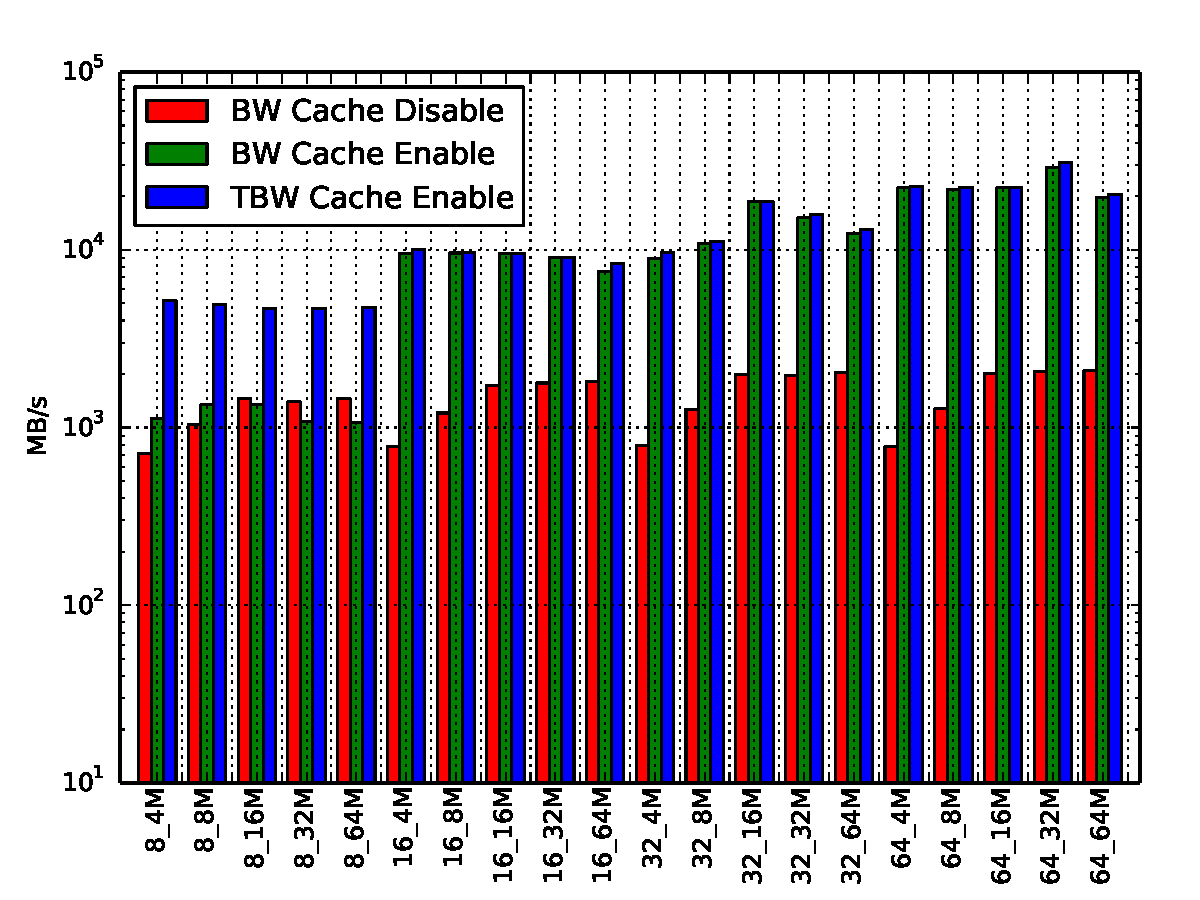
\includegraphics[width=0.95\columnwidth]{figures/coll_perf_32GB_30sec_bw}
  \caption{coll\_perf perceived bandwidth for all combinations of <aggregators>\_<coll\_bufsize>.} % The figure also shows the theoretical bandwidth (TBW) when the cache is not flushed.}
  \label{figure: collperf-bw}
\end{figure}
First of all, we can observe that for most of the experiments the aggregate bandwidth when using the cache is higher than the bandwidth measured when using only the global file system. In particular, we can reach a peak performance of about 20~GB/s, compared to the 2~GB/s of the standard case (BW Cache Disabled), which gives a ten fold improvement. Second, when the number of aggregators is equal to 8, we notice a reduced performance, as the synchronisation cost cannot be completely hidden.

\begin{figure}[b!]
  \centering
  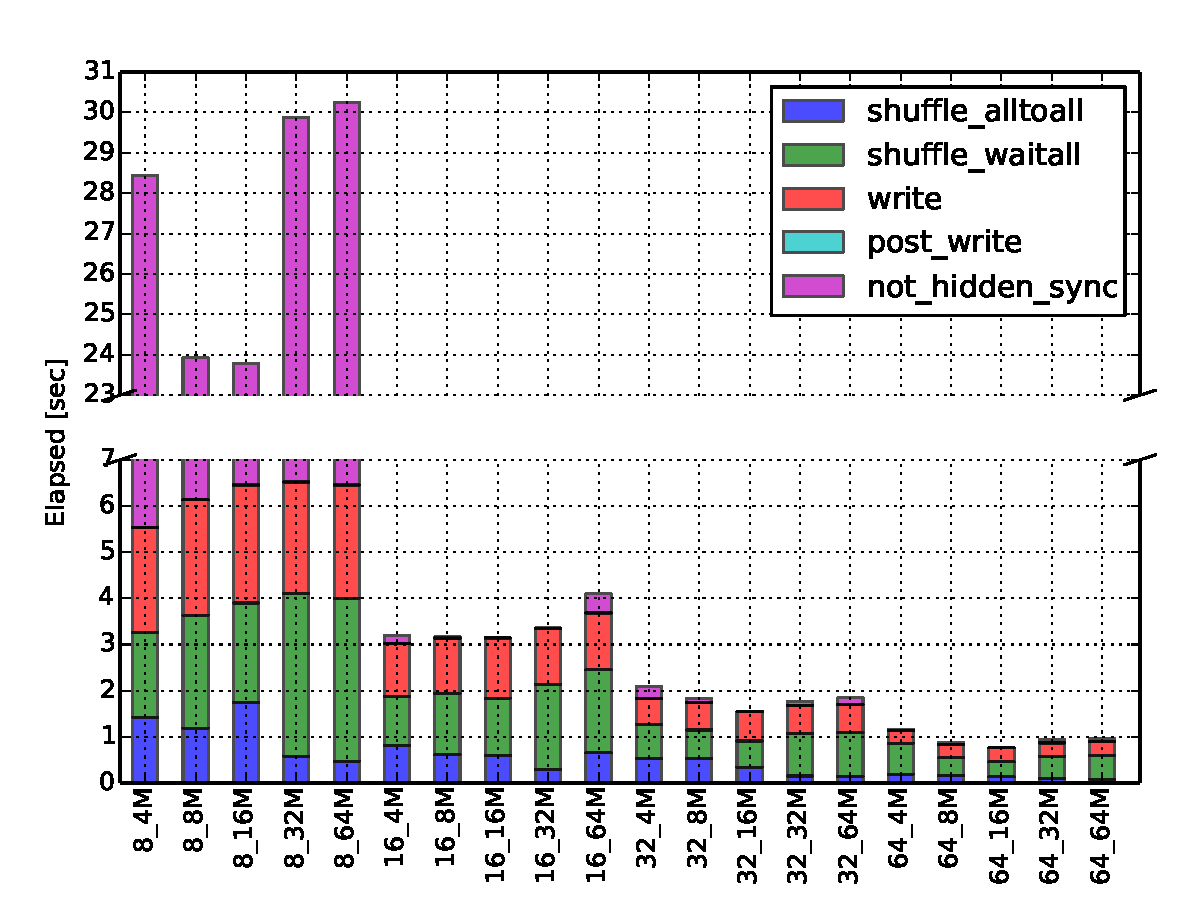
\includegraphics[width=0.95\columnwidth]{figures/coll_perf_32GB_30sec_elapsed_enable}
  \caption{coll\_perf collective I/O contribution breakdown when cache is enabled.} % When the number of aggregators is 8 we clearly see the effect of synchronisation.}
  \label{figure: collperf-elaps-enable}
\end{figure}
The effect of the non-hidden cache synchronisation (not\_hidden\_sync) is shown in Figure~\ref{figure: collperf-elaps-enable}. This figure presents the collective I/O performance breakdown for all the components shown in Figure~\ref{figure: coll_io_impl}. As we can see, although the theoretical bandwidth (TBW Cache Enable) peaks at 4~GB/s (Figure~\ref{figure: collperf-bw}), the measured bandwidth (BW Cache Enable) can be even worse than the standard case (BW Cache Disable). This happens because the cache data cannot be flushed to the global file system quickly enough. In all the other experiments, the perceived and theoretical bandwidth are well aligned.

\begin{figure}[htb]
  \centering
  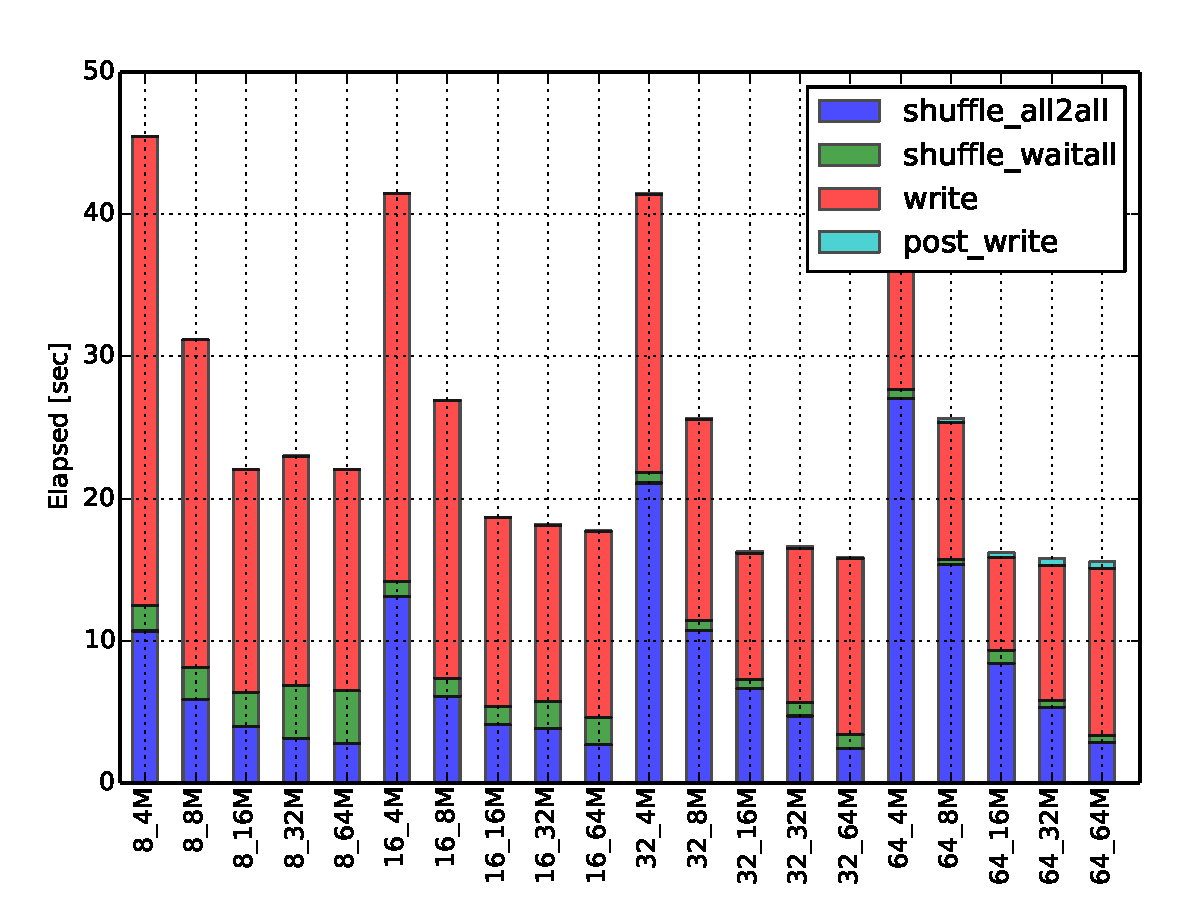
\includegraphics[width=0.95\columnwidth]{figures/coll_perf_32GB_30sec_elapsed_disable}
  \caption{coll\_perf collective I/O contribution breakdown when cache is disabled.}
  \label{figure: collperf-elaps-disable}
\end{figure}

As already said in the previous sections, our SSDs based approach can also help to reduce the global synchronisation cost in the extended two phase I/O algorithm at the base of collective I/O.
In fact, by comparing Figures~\ref{figure: collperf-elaps-enable} and~\ref{figure: collperf-elaps-disable}, we see that the global synchronisation costs in collective I/O, represented by \codeword{MPI\_Alltoall()} (shuffle\_all2all) and \codeword{MPI\_Allreduce()} (post\_write) are consistently reduced when using the cache.

Finally, we observe that most of the times, when using the cache, larger collective buffers do not produce large performance improvements. This means that we can achieve good performance with small buffers and thus reduce the memory pressure of collective write operations on compute nodes.

\subsection{Flash-IO}
\label{subsec: flash}
Flash-IO is the I/O kernel of the Flash application. Flash is a block-structured adaptive mesh hydrodynamics code. The computational domain is divided into blocks which are distributed across the processors. Typically a block contains 16 zones in each coordinate direction (x,y,z) and a perimeter of guard cells (presently 4 zones deep) to hold information from the neighbors. The application writes three files using the parallel HDF5 library: a checkpoint file, a plot file without corner data and a plot file with corner data. The checkpoint file is the biggest of the three and consumes the majority of the I/O time. In our configuration the checkpoint file contains 80 blocks/process and each of the 16 zones/block contains 24 variables encoded with 8bytes (768~KB/proc/block). Therefore, the total size is slightly bigger than 30~GB (including metadata).

\begin{figure}[t!]
  \centering
  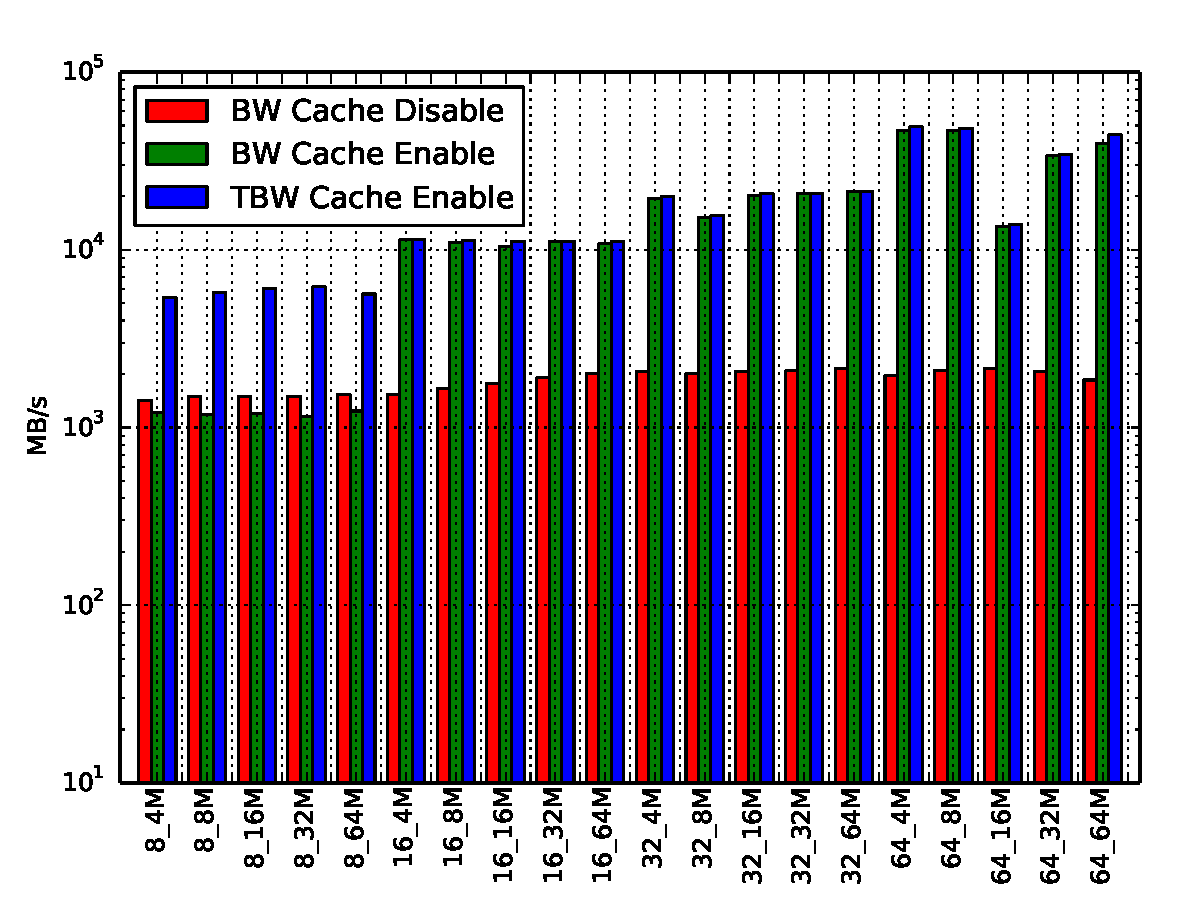
\includegraphics[width=0.95\columnwidth]{figures/flash_32GB_30sec_bw}
  \caption{Flash-IO perceived bandwidth for all combinations of <aggregators>\_<coll\_bufsize>.} %The figure also shows the theoretical bandwidth (TBW) when the cache is not flushed.}
  \label{figure: flash-bw}
\end{figure}

Figure~\ref{figure: flash-bw} shows the write bandwidth perceived by Flash-IO for all the experiments performed in the different cases under study. Similarly to coll\_perf, when the cache is enabled we can hide the cache synchronisation cost for most of the experiments. Once again, like in the previous case, when the number of aggregators is equal to 8 we have a mismatch between the perceived and the theoretical bandwidth. For Flash-IO the peak bandwidth is about 40~GB/s when using 64 aggregators and 4~MB collective buffer size, against the 2~GB/s measured when writing directly to the parallel file system.
\begin{figure}[htb]
  \centering
  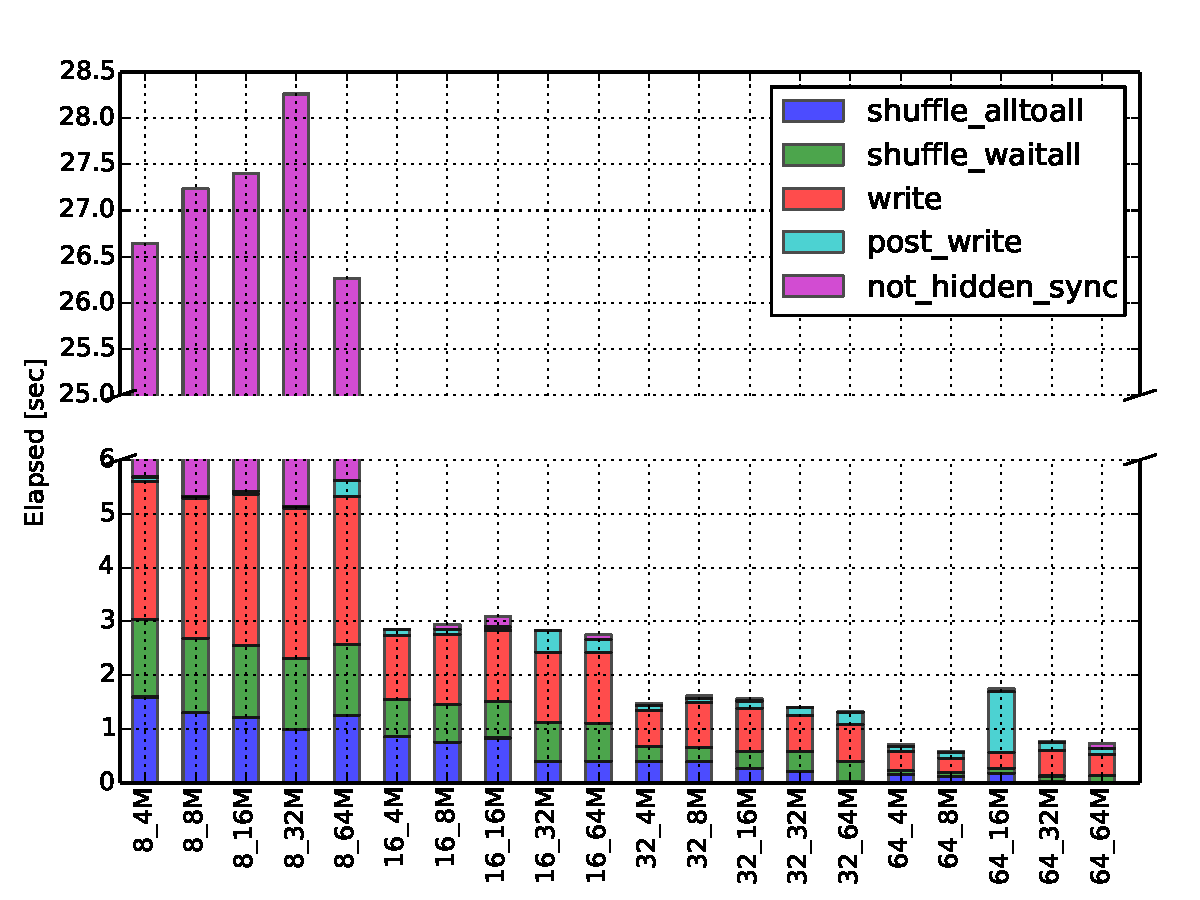
\includegraphics[width=0.95\columnwidth]{figures/flash_32GB_30sec_elapsed_enable}
  \caption{Flash-IO collective I/O contribution breakdown when cache is enabled.}
  \label{figure: flash-elaps-enable}
\end{figure}

Figure~\ref{figure: flash-elaps-enable} shows the effect of cache usage on the different collective I/O performance contributions. We can clearly see that when the number of aggregators is equal to 8 the cache synchronisation cannot be completely hidden, causing the bandwidth mismatch previously observed in Figure~\ref{figure: flash-bw}. Furthermore, like in the coll\_perf case the global synchronisation contributions can be reduced when using the cache, and so can the memory pressure on the compute nodes.
\begin{figure}[htb]
  \centering
  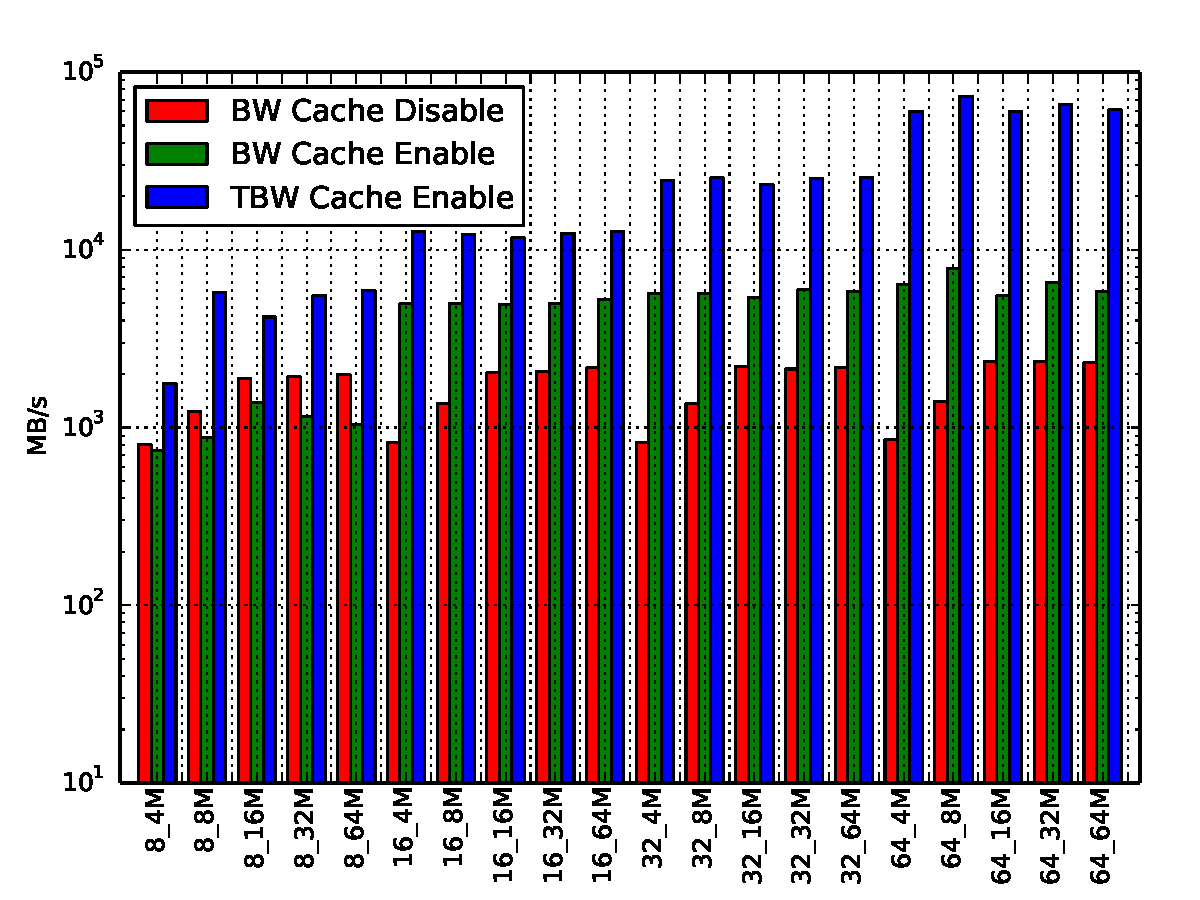
\includegraphics[width=0.95\columnwidth]{figures/ior_32GB_30sec_bw}
  \caption{IOR perceived bandwidth for all combinations of <aggregators>\_<coll\_bufsize>.} %The figure also shows the theoretical bandwidth (TBW) when the cache is not flushed.}
  \label{figure: ior-bw}
\end{figure}
Nevertheless, for the 64 aggregators and 16~MB collective buffer size configuration the global synchronisation overhead associated to \codeword{MPI\_Allreduce()} (post\_write) has a larger value. The outlier causes a strong reduction in the write bandwidth, although we can still achieve more than 10~GB/s. This indicates that the effect of global synchronisation when using the cache can be even more severe, due to the much higher bandwidth achievable compared to the standard global file system approach.

\subsection{IOR}
\label{subsec: ior}
We tested IOR when writing collectively to a shared file. Each of the 512 MPI processes writes one 8~MB block of data for each of the 8 segments, that is, a 32~GB file during every test.
%\todo[inline]{remove standard deviation explanation and focus on the last part where the real reason for reduced performance is exposed. explain that add one additional read and one additional write is making things worse when using a small number of SSD/aggregators. improve figures adding bars for synchronization cost separately. add a reference to the statement that large systems might not be able to write concurrently to all the available I/O targets.}
%\todo[inline]{reading data back from the cache: illustrate problems related to additional metadata information required (example ADIOS does this using a custom binary format). describe this in related or future work.}
As for the previous two benchmarks, Figure~\ref{figure: ior-bw} shows the write bandwidth perceived by IOR. Nevertheless, unlike the previous benchmarks, in IOR we also take into account the non-hidden synchronisation cost coming from the last write phase. In this case, the peak bandwidth when using the cache can reach about 6~GB/s versus the 2~GB/s of the standard collective write to the global file system. We can also see that the theoretical bandwidth is aligned with the figures presented for coll\_perf and Flash-IO. In fact, although we can hide cache synchronisation costs for the three intermediate write phases in IOR, the fourth write phase will limit the peak performance.

Figures~\ref{figure: ior-elaps-enable} shows the collective I/O cost breakdown for all the time contributions. 
\begin{figure}[htb]
  \centering
  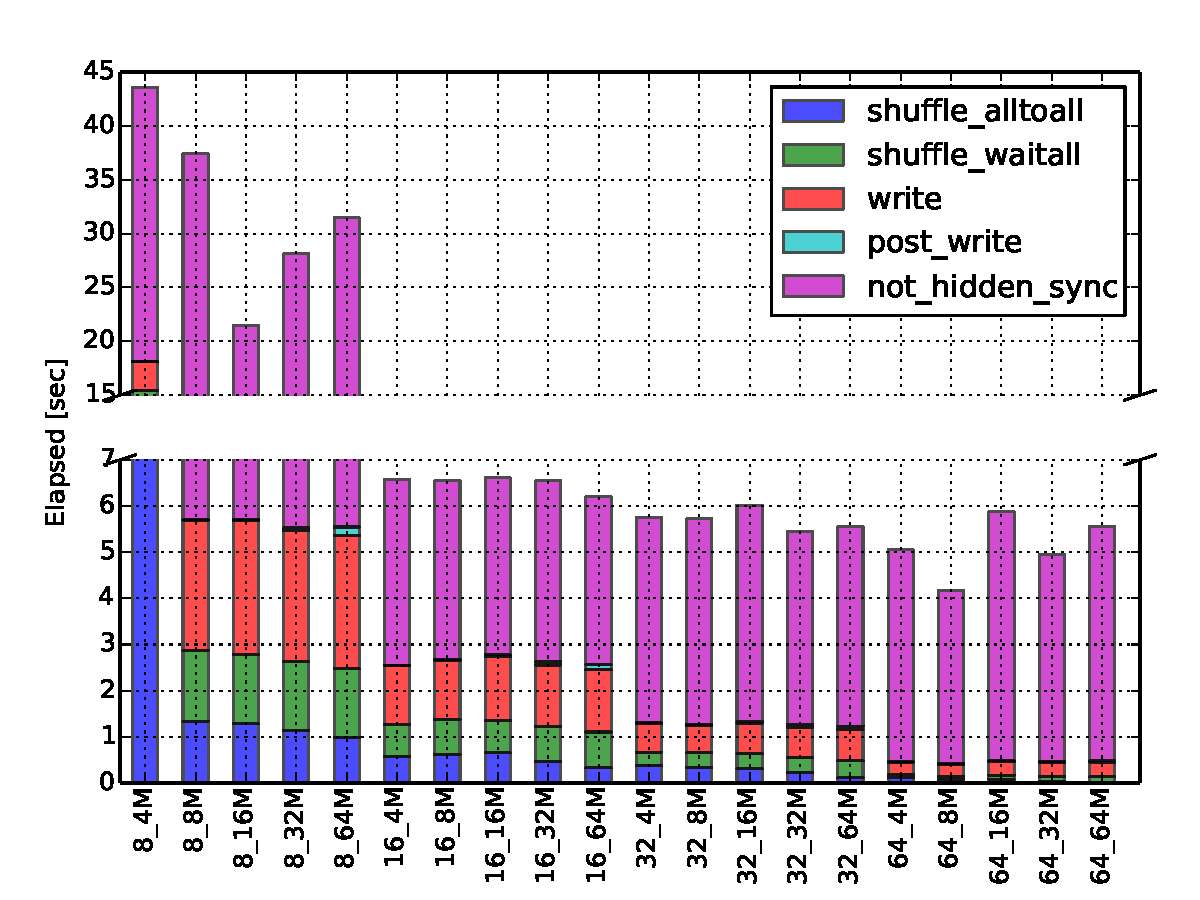
\includegraphics[width=0.95\columnwidth]{figures/ior_32GB_30sec_enable}
  \caption{IOR collective I/O contribution breakdown when cache is enabled.}
  \label{figure: ior-elaps-enable}
\end{figure}
In this figure we can clearly observe the not\_hidden\_sync term preventing IOR from achieving higher performance. This is added to the other time contributions and corresponds to the term $T_s(k)-C(k+1)$ reported in Equation~\ref{formula: bw}. In our specific case, $k = 4$ and $C(4+1) = 0,$ meaning that the total write time is accounting for the whole $T_s(4)$ term.

